%
% Charset: utf8
% Content type: Plain LATEX
% Content: This chapter describes how the bootloader 'Barebox' functions and
%          how to modify things to get Barebox to work properly.
%
% Copyright Jürgen Beisert <jbe@pengutronix.de>, 2011
%
% This work is licensed under the Creative Commons Attribution 3.0 Unported License.
% To view a copy of this license, visit:
%           http://creativecommons.org/licenses/by/3.0/
% or send a letter to:
% Creative Commons, 444 Castro Street, Suite 900, Mountain View, California, 94041, USA.
%
% Refer the file CREDITS for all people working on this document.
%
% This file content will be part of the "OSELAS.BSP-Pengutronix-Mini2440-Quickstart.pdf"
%
% Note: This document uses some externaly defined LATEX commands. If you try to
% run LATEX only on this file it will fail due to the absense of these commands
% All these new commands are starting with 'ptxdist'.
%

\section{Notes About the Bootloader Barebox}	\label{sec:bareboxnotes}

Everything mentioned here (variable names and file names) in the run-time
environment that Barebox uses, is for convenience only. The developers of Barebox
decided to provide a generic run-time environment that satisfies the most
common requirements. All descriptions below will refer to this generic
run-time environment and it's behaviour.

There are no restrictions in how to adapt this environment for one's own
needs. How Barebox enters it's shell is compiled-in. Changing the
\texttt{/env/bin/init}, allows one to modify Barebox's behaviour.

%
% Idea: Describe the way from the /env/bin/init script to the booting kernel
% - where are the parameters from
% - how to change the boot source
%

\subsection{Run-Time Environment}			\label{sec:bbenv}

The Barebox binary handles only target initialization and provides device
drivers and various commands to do things after the initialization. It is up to
the user to use these features to make her/his target work. This works on a
shell code base. For example, Barebox tries to run the \texttt{/env/bin/init}
script right after the initialization is finished. This file is expected
as a part of the environment.

From the technical point of view, the Barebox environment is a simple
archive which contains files and directories. At startup, this archive will
be extracted to the \texttt{env/} directory and can be used afterwards
on a regular file base. Note: the \texttt{/} directory in Barebox is a RAM
filesystem.

Barebox always tries to load the user environment archive from the registered
persistent media first (aka "user env"). If this fails, Barebox defaults to the
default compiled-in environment archive.

The compiled-in default environment archive is a read only archive defined at
compile-time of Barebox.

The \textit{user env} can be changed at any point of time.

\subsubsection{Run-Time Environment (\textit{env}) and how it is controlled by Barebox}

When starting from a totally clean system (e.g. NAND flash is empty) and if
you do an \texttt{update -t barebox -d nand} to bring in the Barebox bootloader
into the NAND flash and then reset the mini2440, Barebox will use its default
compiled-in environment because the \textit{user env} is still empty. To change
the run-time Barebox environment, on the target, one can do \texttt{edit /env/config}
(to make the changes), \textit{CTRL D} (to store the changes to the RAM disk and
leave the editor) and a \texttt{saveenv} (to save the changes to the
\textit{user env}). The next time we boot the mini2440, the \textit{user env}
takes priority. Note: the default Barebox environment has not been changed.

Here a graphic to show the process:

\centerline{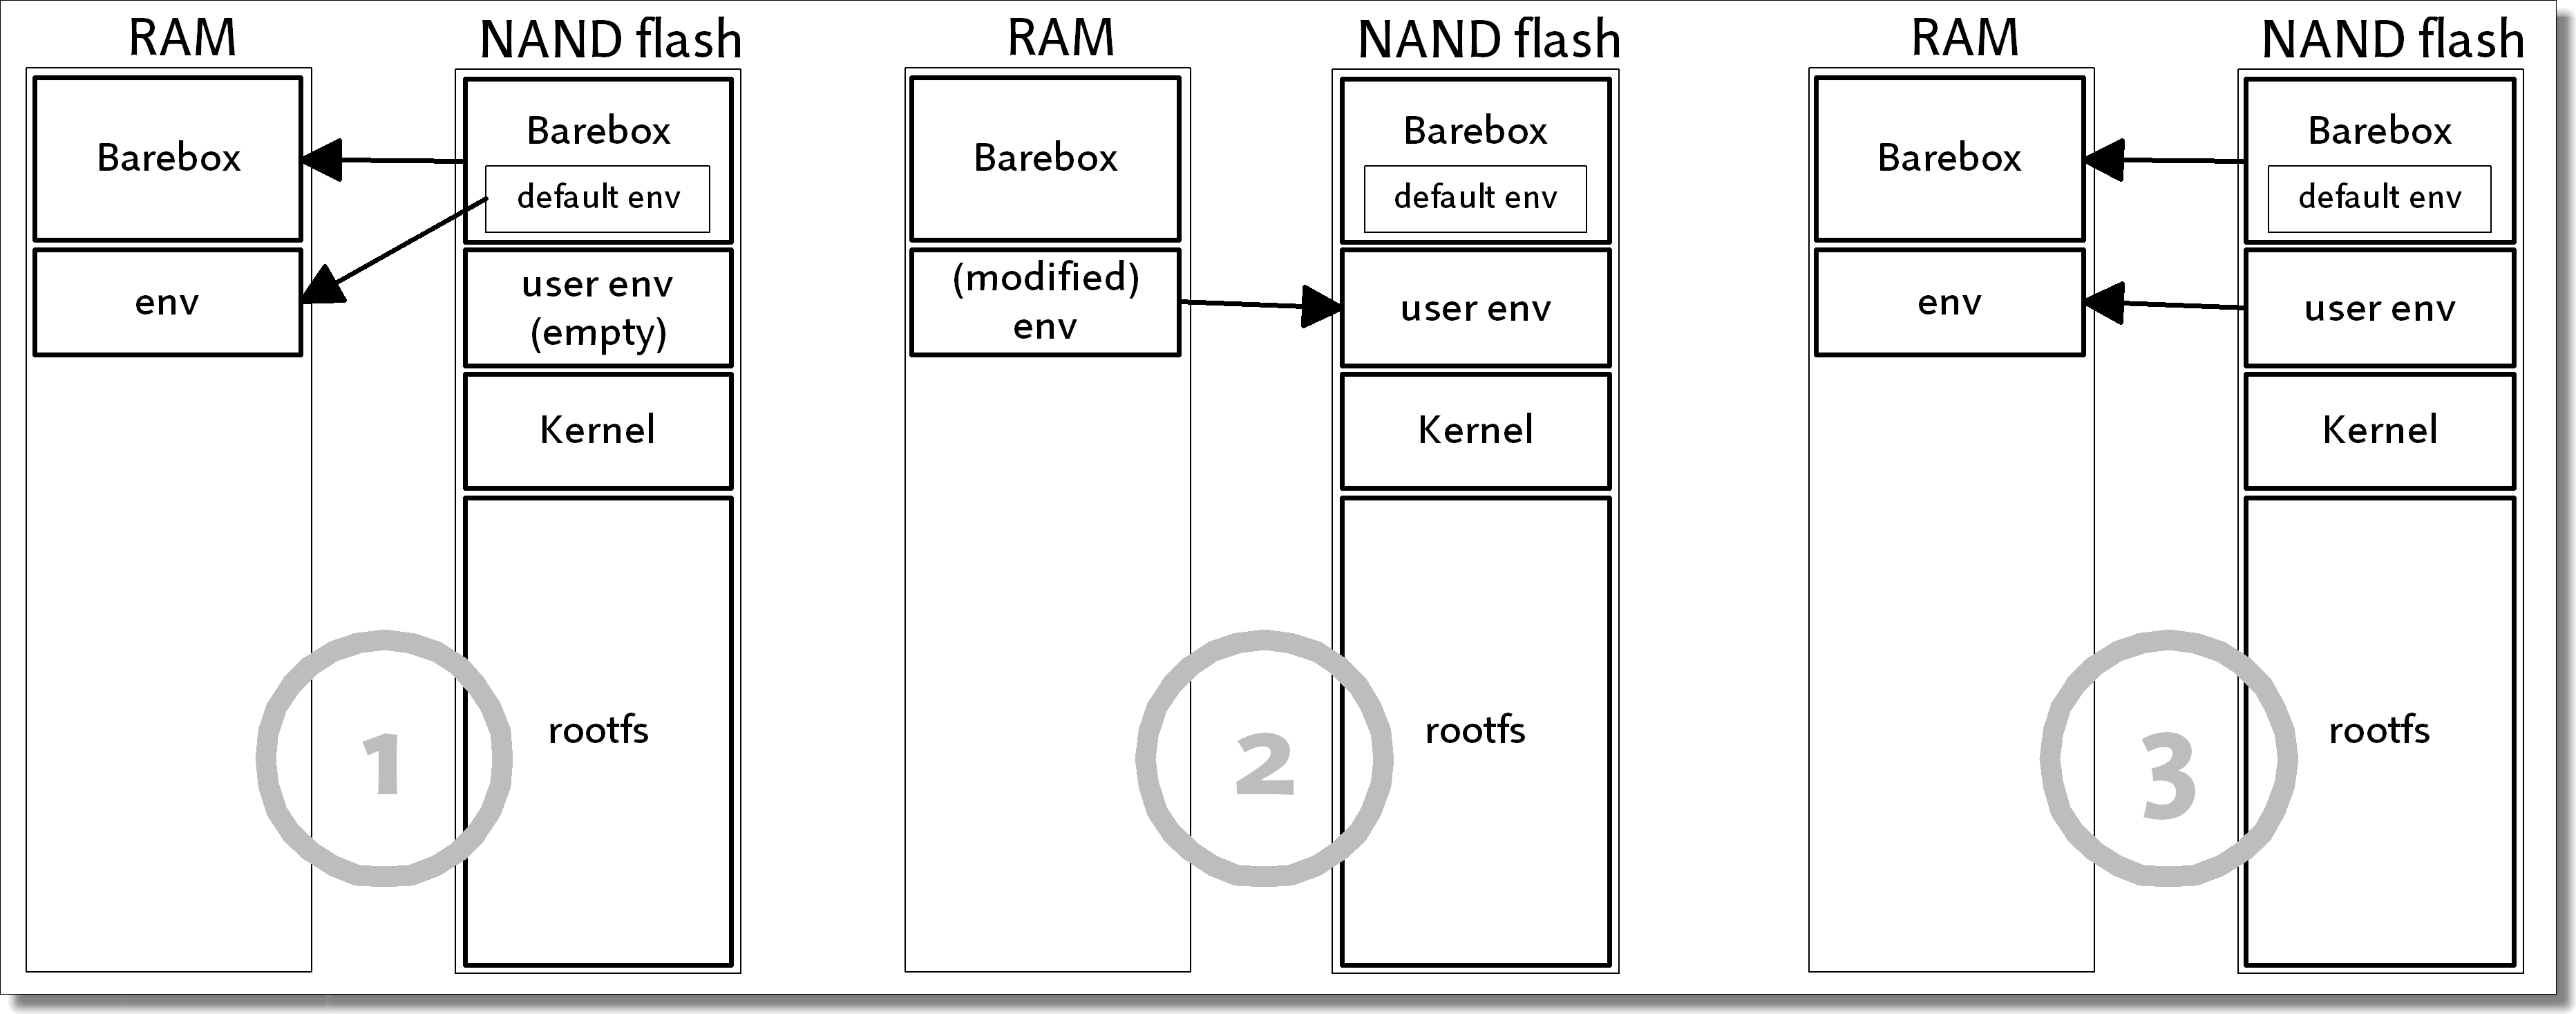
\includegraphics{OSELAS.BSP-Pengutronix-Mini2440/documentation/plain_sources/default_versus_user_env.png}}

\begin{itemize}
	\item state 1: the 1st boot. Barebox runs in RAM and loads the
	      \textit{env} from the default compiled-in environment due to the
	      \textit{user env} is still empty
	\item state 2: the user changes the \textit{env} and saves it. Now, the
	      \textit{user env} is no longer empty
	\item state 3: At the next system start Barebox now ignores the default
	      compiled-in environment and loads its \textit{env} from the
	      \textit{user env}
\end{itemize}

The above method is appropriate for minor changes in the Barebox environment. For
major env changes it is suggested that we modify the environment files in the board
support package instead of on the target. On our host it's easier to change these files
(for example with our favourite editor instead of the simple editor embedded in
Barebox) and these changes remain, should we want to re-build everything again.

The environment is a collection of files from different locations in the board
support package. One location is the \texttt{configs/\ptxdistPlatformName /barebox-64m-env/}.
Another location is \texttt{\ptxdistPlatformDir /build-target/barebox-\ptxBareboxRev /defaultenv/}.
The second location contains the more generic shell scripts, while the first
location contains user specific settings. If we intend to change the generic shell
scripts, it's easier to copy them to the \texttt{configs/\ptxdistPlatformName /barebox-64m-env/}
location instead of modifying them at their original path (as this modification would
be lost, if we run \texttt{ptxdist clean}). The files at
\texttt{configs/\ptxdistPlatformName /barebox-64m-env/} takes priority over the
one from the \texttt{\ptxdistPlatformDir /build-target/barebox-\ptxBareboxRev /defaultenv/}
if files with the same name exits.

After such a change we should run:

\begin{ptxshell}[escapechar=|]{^}
|\$| ptxdist clean barebox
|\$| ptxdist go
|\$| ptxdist images
\end{ptxshell}

This rebuilds Barebox and includes the changed default compiled-in environment.

Next, make these files available for download via network/TFTP:

\begin{ptxshell}[escapechar=|]{^}
|\$| cp |\ptxdistPlatformDir |images/barebox-image /tftpboot/barebox-mini2440
\end{ptxshell}

Now,

\begin{ptxshell}[escapechar=|]{^}
mini2440:/ update -t barebox -d nand
\end{ptxshell}

together with its new compiled-in default environment. But at the next system
start also this new Barebox would use the \textit{user env} if it is still present.
To make it use the new compiled-in default environment we must either remove
the \textit{user env} with:

\begin{ptxshell}[escapechar=|]{^}
mini2440:/ erase /dev/nand0.bareboxenv.bb
\end{ptxshell}

or update the \textit{user env} with the prepared archive from the last build:

\begin{ptxshell}[escapechar=|]{^}
|\$| cp |\ptxdistPlatformDir |images/barebox-default-environment /tftpboot/barebox-default-environment-mini2440
\end{ptxshell}

\begin{ptxshell}[escapechar=|]{^}
mini2440:/ update -t bareboxenv -d nand
\end{ptxshell}


% Idea: Describe the components of the default environment provided by the
% Barebox source tree. What variables/scripts are used and their meaning

\subsection{How does the Partitioning Work in Barebox}	\label{sec:bbpartitioning}

Partitioning is a way to handle large media in smaller logical units. This
simplifies updates of different components and leaves others untouched. For
example, one can update the kernel to fix a bug in a driver but keep the
root filesystem unchanged. Also, redundant boot can be realized with more than
one partition per component.

%
% Idea: Add a description what "redundant boot" means
%

Barebox uses partitioning of the available persistent media (for example, NOR
or NAND flash, but also harddisks or SD cards) to handle and store the
required parts to make a target work.

Some of the available persistent media can store it's partition information on
the media itself. For example hard disks, compact flash cards or SD cards can
provide their own partition table.

In this case, Barebox can read back this table from the media and handle
these partition's sizes and locations in a correct manner.

But, there are still some media that do not provide this kind of partition table.
The well known plain flash devices (of type NOR or NAND) are such candidates.
These devices need slightly different handling. The most common method the
kernel uses is the \textit{Command line partition table parsing} for the MTD
(Memory Technology Devices) devices. A user gives a kernel parameter with the
list of names and sizes that describes the partition layout of the
corressponding flash memory.

%
% How to describe this? If Barebox do not use the plain flash, there is no need
% to partitioning it. This is the case if a target comes with NOR _and_ NAND
% memory and starts from the NOR. If Barebox does not touch the NAND flash memory,
% there is no need to partition it. On the other hand, for NOR flash we need some
% kind of partitioning. In this case, because we are starting from this memory,
% we must protect the bootloader from accidental erasure.
%

Barebox uses the same syntax to describe the partition and kernel layout. So,
a user only has to define the layout once. It will be shared between Barebox
and the Linux kernel. If one doesn't use consistent layout, one could destroy
the data in one partition by changes in another parition.

This partition layout string is defined to:

\begin{ptxshell}[escapechar=|]{^}
<size>(<name>)[,<size>(<name>)[,<size>(<name>)]...]
\end{ptxshell}

\texttt{<size>} is a number followed by its unit. The unit can be \texttt{k} for
\textit{kilobyte}, \texttt{M} for \textit{megabyte} and \texttt{G} for
\textit{gigabyte}. For \texttt{<size>} also the special letter \texttt{-}
can be given. This means, fill the remaining space up to the end of the media. The
\texttt{<name>} can be anything one likes, but must not contain any spaces!

Here is the most common partition layout configuration:

In Barebox's run-time environment it looks like:

\texttt{256k(barebox),64k(bareboxenv),2048k(kernel),-(root)}

\begin{itemize}
	\item bootloader itself (\textit{barebox}): this binary brings up the target
	      after power on or reset
	\item persistent environment (\textit{bareboxenv}): used by Barebox to bring up
	      the whole system in the way that the user has configured it
	\item operating system (\textit{kernel}): the kernel image, Barebox will load
	      and run it
	\item root filesystem (\textit{root}): used by the kernel as the root
	      filesystem
\end{itemize}

The size and location of some of these partitions can be modified at run-time
via the variable \texttt{nand\_parts} in the \texttt{env/config} file. Here the
user can increase the kernel partition, or add more partitions to the
\textit{free part} of the list.

However, two of the listed partitions are special: the location and size of
the bootloader (\textit{barebox}) partition and of the run-time environment
(\textit{bareboxenv}) partition.
%
% "[...] \textbf{AND} the location of the kernel."
%
% No, this partition is not fixed in its location. It just starts after the
% 'bareboxenv' partition. OK!
%

These must be known soon after reset. So, we have a chicken/egg problem: to
read the persistent environment, Barebox must know where the persistent environment
is located. To do so, Barebox initially creates the \textit{barebox} and
\textit{bareboxenv} partitions and after loading the persistent environment
Barebox then adds the \textbf{remaining} partitions based on the
\texttt{nand\_parts} variable.

This handling implies the internally registered partitions for Barebox and the
persistent environment must be the same in size and location as the partitions
described in the \texttt{nand\_parts} variable.

This then means, if one would like to change the size of the \textit{barebox}
or the \textit{bareboxenv} partitions, she/he must change the platform source
code \textbf{and} the \texttt{nand\_parts} variable.

Here an example for a partition setup in the run-time environment:

\begin{ptxshell}[escapechar=|]{^}
nand_parts="256k(barebox),64k(bareboxenv),2048k(kernel),-(root)"
\end{ptxshell}

It corresponds to the following NAND partition layout:

\centerline{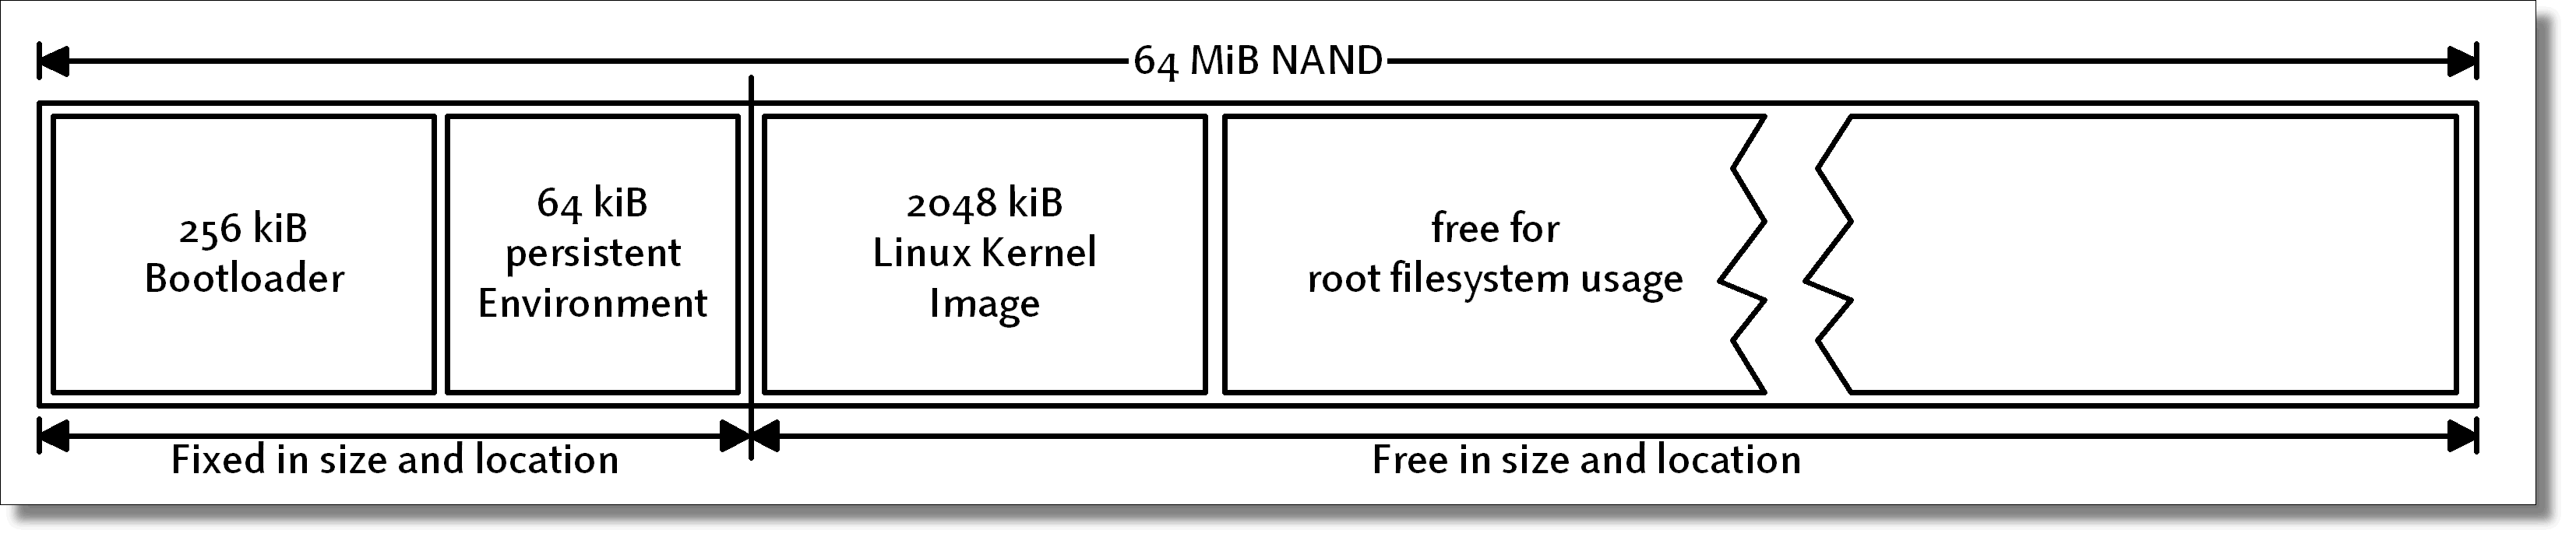
\includegraphics[width=16cm]{OSELAS.BSP-Pengutronix-Mini2440/documentation/plain_sources/partitioning.png}}

This setup defines

\begin{itemize}
 \item 256 kiB for the bootloader (\textit{barebox}) at the beginning of the
  persistent media.
 \item 64 kiB for the persistent environment (\textit{bareboxenv}) following
  the bootloader partition
 \item 2 MiB for the kernel (\textit{kernel})
 \item the remaining space on the persistent media for the root filesystem
  (\textit{root})
\end{itemize}

For the Mini2440 the platform source code is located in:

\texttt{platform-mini2440/build-target/barebox-<version>/arch/arm/boards/mini2440/mini2440.c}

and looks like this:

\begin{ptxshell}[escapechar=|]{^}
[...]
      /* ----------- add some vital partitions -------- */
   devfs_del_partition("self_raw");
   devfs_add_partition("nand0", 0x00000, 0x40000, PARTITION_FIXED, "self_raw");
   dev_add_bb_dev("self_raw", "self0");

   devfs_del_partition("env_raw");
   devfs_add_partition("nand0", 0x40000, 0x10000, PARTITION_FIXED, "env_raw");
   dev_add_bb_dev("env_raw", "env0");
[...]
\end{ptxshell}

Please ensure after changing any of the "Fixed in size and location" partitions
that Barebox is re-compiled and re-flashed to keep the compiled-in environment
in sync with the platform source code.

Also consider: for the partitions that are free in size and location, you can
change these settings at run-time and store it to the persistent environment.
But, if this persistent environment gets lost Barebox will default to the
compiled-in environment. If this compiled-in environment has different
partition sizes and locations, error messages will occur. This is because
reading from partitions with wrong settings in size and location will fail.

So, the best procedure is to change the compiled-in environment to ensure the
partition layout is always consistent, even if the modified persistent
environment gets lost.

\section{NFS with PTXdist and Barebox}

NFS stands for \textit{\textbf{N}etwork \textbf{F}ile\textbf{S}ystem}. It is one
way to export a local filesystem content via network to another host. In our case
we can use it to simulate a root filesystem for our target. This simplifies application
development for the Mini2440. We do not have to change anything locally on the
Mini2440. As our target is using our local host's filesystem, we can also change
everything locally and it will be visible at target's side instantly.

Starting with \ptxdist{}-2012.10.0 there is more than one choice how to get
the network based development to work.

\begin{itemize}
	\item a user mode NFS daemon, coming with \ptxdist{}
	\item a classic NFS daemon, running on our development host
\end{itemize}

\subsection{Classic NFS daemon}

Configuring and running the classic NFS daemon requires root permissions on the
development host: files owned by root must be modified and system services must
be run. If we don't have root permissions, the user-mode NFS daemon is a useful
alternative. Refer \ref{sect:usermode_nfs}.

What we need at our host's side:

\begin{itemize}
	\item NFS server support in our Linux kernel
	\item NFS utils
	\item the \texttt{portmap} tool
\end{itemize}

It depends on the distribution we are using, how to get and enable this feature on
our host.

To get these components on a Ubuntu based system we just have to enter:

\begin{ptxshell}[escapechar=|]{^}
|\$| sudo apt-get install nfs-kernel-server nfs-common portmap
\end{ptxshell}

The last two may not be required for a NFS server, but if you decide to install a
NFS client on the Ubuntu box or need to do any troubleshooting later, you will
need them.
% FIXME: AFAIK 'portmap' is always required as it manages the network ports to be used

First thing is to enable the export of specific parts of the host's local filesystem.
This should be done \textbf{very} carefully, because:

\begin{itemize}
	\item we must export the required filesystem parts in a very unsafe manner
	\item typos in the export's controling file may results into very funny and
		confusing error messages
\end{itemize}

The "unsafe manner" means, we allow any \textit{root} user on the remote system
using our local filesystem also to be the root user on our host! This is a huge
security hole, if more parts of the local filesystem gets exported than intended.

\ptxdist{} creates one directory intended for NFS root filesystem export when building
the board support package:

\begin{ptxshell}[escapechar=|]{^}
|\$|  ls |\ptxdistPlatformDir |root
bin  dev  etc  home  lib  mnt  proc  root  run  sbin  sys  tmp  usr  var
\end{ptxshell}

If we are a little bit paranoid we should only export exactly this one directory. The
best way to know what directory path has to be used to export exactly this directory
we can follow these steps:

\begin{ptxshell}[escapechar=|]{^}
|\$| cd |\ptxdistPlatformDir |root
|\ptxdistPlatformDir |root|\$| pwd -P
/home/me/|\ptxdistBSPName |/|\ptxdistPlatformDir |root
\end{ptxshell}

The path, the \texttt{pwd} command outputs is the one we should export at our local
host and our Mini2440 must mount at runtime to get access to this directory.

\begin{important}
Exporting this specific directory presumes the directory must already exist when the export
is enabled. Exporting first and then building the board support package (which creates the
directory at this point of time) does not work as expected. Every \texttt{ptxdist clean; ptxdist go}
requires to re-export this directory.\\
To be less dependend on the build state of the board support package, the BSP's directory
could be exported instead: \texttt{/home/me/\ptxdistBSPName }
\end{important}

But step by step. \textit{Export} first:

The file to be modified is the \texttt{/etc/exports}. This file is used by the NFS related
tools to know what parts of the filesystem should be exported and how it should be exported.

In our case we add the following line to this file:

\begin{ptxshell}[escapechar=|]{^}
/home/me/|\ptxdistBSPName |/|\ptxdistPlatformDir |root *(rw,no_root_squash,sync,no_subtree_check)
\end{ptxshell}

What does it mean: First part of the line is the to be exported directory. Second part is,
who is allowed to use this directory. In the line mentioned above the asterisk ('\texttt{*}')
means \textit{everybody}. Here we can use an IP range instead of an asterisk to make the
security hole a little bit smaller. Or, even smaller by only allowing one IP address.
The third part are the permissions the remote host has
on our locally exported path. \texttt{rw} means read write permission. The opposite is
\texttt{ro} which means read only. But in our case we need the \texttt{rw} in order to use
the exported directory for our root filesystem requirements.

Note: Do not add any white space between the asterisk/IP range and the left parenthesis
starting the permission or you will get confusing error messages.

Most of the time there is no user management at our targets. Or to be more precise: most of
the time only one user is required to make the target work as expected. This is always the
user \textit{root}. To allow this root user at the target side to touch all files in our exported
directory the parameter \texttt{no\_root\_squash} must be given. But be aware: In this
case the remote root user is also the root user on our host! Do you feel the risk? ;-) That's why
only to export the required directory and nothing more.

If the NFS service is not running on our host yet, it's now time to run it:

\begin{ptxshell}[escapechar=|]{^}
|\$| sudo /etc/init.d/nfs-kernel-server start
\end{ptxshell}

Note: This step can differ on other distributions.

If the NFS service is already running, we can force to export all directories listed in
\texttt{/dev/exports} by running:

\begin{ptxshell}[escapechar=|]{^}
|\$| sudo exportfs -rv
\end{ptxshell}

To check the current export state we can simply run a:

\begin{ptxshell}[escapechar=|]{^}
|\$| sudo exportfs -v
/home/me/|\ptxdistBSPName |/|\ptxdistPlatformDir |root
	<world>(rw,wdelay,no_root_squash,no_subtree_check)
\end{ptxshell}

Note: Sometimes the list of options differ from the options we give in
\texttt{/etc/exports}. These options are the default settings the NFS service
is used if not otherwise set.

\texttt{<world>} means here the asterisk ('\texttt{*}').

Now is everything prepared at the host's side. Next step is to instruct our
Mini2440 to use the new host's feature. Refer section \ref{sec:networkmem} how
to do so. The variable \texttt{nfsroot} must be setup in accordance to the
exported filesystem on our host.

Even if we export

\begin{ptxshell}[escapechar=|]{^}
/home/me/|\ptxdistBSPName |
\end{ptxshell}

on our host (to avoid the \texttt{ptxdist clean; ptxdist go} issue mentioned
in the WARNING above), our Mini2440 must always use the full path:

\begin{ptxshell}[escapechar=|]{^}
nfsroot=/home/me/|\ptxdistBSPName |/|\ptxdistPlatformDir |root
\end{ptxshell}

After we have a working NFS system all that is required is a power-up on the
Mini2440, connected to our host, to enable sharing of the root file system.

After login to our target we can now look at any of the files in
\texttt{\ptxdistPlatformDir root}, for example:

On the server (host):

\begin{ptxshell}[escapechar=|]{^}
/home/me/|\ptxdistBSPName |/|\ptxdistPlatformDir |root/etc/fstab
\end{ptxshell}

and on the target (Mini2440)

\begin{ptxshell}[escapechar=|]{^}
/etc/fstab
\end{ptxshell}

We should see that the contents of these files are the same. Also, we can
change this file’s contents from our target or from our host AND see the
changes appear on the other device.

\subsection{Troubleshooting}

If towards the end of the kernel boot process you get this message:

\begin{ptxshell}[escapechar=|]{^}
VFS:  Unable to mount root via NFS, trying floppy
VFS:  Cannot open root device “nfs” or unknown-block(2,0)
\end{ptxshell}

Don’t panic!

Have a look in \texttt{/var/log/syslog} on the server and if you see a
message like this:

\begin{ptxshell}[escapechar=|]{^}
Jun 15 21:30:09 my-desktop mountd[1716]: refused mount request from 192.168.1.230 for
/home/me/|\ptxdistBSPName |/|\ptxdistPlatformDir |root (/): not exported
\end{ptxshell}

Have a \textbf{real close} look and see that you haven’t made a mistake. Check
again the directory the server exports and also check the content of the \texttt{nfsroot}
variable. The start of the path must match exactly. Any typo will result into this
kind of failure.

\subsection{Usermode NFS daemon}					\label{sect:usermode_nfs}

The advantages of the user-mode NFS daemon are:

\begin{itemize}
	\item no Linux kernel support required
	\item no root permissions required
	\item less painful to configure
	\item less security issues
	\item all exported files have correct permissions and owners (at least from
	the target's point of view)
	\item \ptxdist{} provides everything required to make it work
\end{itemize}

Due to the different behaviour of the user-mode NFS daemon in contrast to the
Linux kernel based classic NFS daemon, the target needs a different setup to
make it work with the user-mode NFS daemon.

From the target's point of view

\begin{itemize}
	\item a fixed path is used to mount the NFS root
	\item different network ports are in use
\end{itemize}

The NFS root path the user-mode NFS daemon exports is just \texttt{/root}. This
simplifies the path to be setup at the target. But as it is a user-mode NFS
daemon it cannot use the standard network ports of the classic NFS daemon. That's
why we need to define different port numbers for the bootloader and the kernel.

The user-mode NFS daemon uses the network port 2049 for the \textit{NFS service
port} and also network port 2049 for the \textit{mountd port}. We must ensure
our target uses these network ports, when it contacts our host.

Putting everything together for the Linux kernel:

\begin{ptxshell}[escapechar=|]{^}
nfsroot="/root,v3,tcp,port=2049,mountport=2049"
\end{ptxshell}

After the setup of the target is done, the next step is to start the user-mode
NFS daemon at our host. Thanks to \ptxdist{} this step is very easy now:

\begin{ptxshell}[escapechar=|]{^}
|\$| ptxdist nfsroot

Mount rootfs with nfsroot=/root,v3,tcp,port=2049,mountport=2049

UNFS3 unfsd 0.9.22 (C) 2006, Pascal Schmidt <unfs3-server@ewetel.net>
/home/me/|\ptxdistBSPName |/|\ptxdistPlatformDir |: ip 0.0.0.0 mask 0.0.0.0 options 5
\end{ptxshell}

Note: if a classic NFS daemon is already running, the user-mode NFS daemon might
conflict with it. If the user-mode NFS daemon terminates with the message:

\begin{ptxshell}[escapechar=|]{^}
bind: Address already in use
Couldn't bind to udp port 2049
\end{ptxshell}

then a classic NFS daemon is still running and should be stopped first.

\begin{important}
Even if the user-mode NFS daemon is used for the NFS root filesystem, currently
a TFTP daemon for downloading the Linux kernel is still required. Maybe future
releases will also remove this dependency.
\end{important}
